\chapter{Methodology}
\label{chap:met}

The primary objective of this research endeavor is to investigate the process of distilling an LLM into a sequence classification model (hereafter referred to as ``the classifier'') and to evaluate the efficacy of this methodology in comparison with alternative approaches. These alternatives include constructing a classifier from the ground up, fine-tuning a pretrained classifier, and implementing a black-box knowledge distillation technique onto an LLM\@. The efficacy of the models under consideration will be quantitatively assessed based on the accuracy of their predictions on a designated test set.

This chapter details the architecture of the student model and its training process. After that, I provide an elaborate description of the experimental setup, which includes the datasets in use, the architecture of the models under examination, the employed knowledge distillation techniques, and the adopted effectiveness metrics. This systematic exposition aims to furnish a clear understanding of the methodologies employed and facilitate a rigorous analysis of their relative merits and demerits in the context of enhancing model performance and efficiency.

The distillation methods proposed is inspired by reviewed black-box LLM distillation methods (\autoref{section:blackbox}). Authors demonstrate how to leverage the deep insights of large models to guide the training of compact models using rationale generated by LLM (\autoref{fig:stepbystep}). This rationales offer a more in-depth insight into the reasoning behind associating an input with a particular output label. Provided approach serves as a foundation for developing a more efficient and effective distillation method tailored specifically for sequence classification models.

\section{Datasets}

The datasets selected for this study specifically chosen for their applicability to the research at hand. The primary criterion for dataset selection is their relevance to classification tasks. Through this targeted dataset selection, the research aims to rigorously evaluate the effectiveness of incorporating rationales into the training process of classification models.

\subsection{Extended Stanford Natural Language Inference (e-SNLI)}

For the exploration of the student model's capabilities in classification tasks, we specifically focus on Natural Language Inference (NLI) datasets within the scope of this research. NLI datasets are pivotal for evaluating the model's proficiency in understanding and processing human language, offering a rich ground for testing its ability to deduce the logical relationship between premises and hypotheses. These datasets consist of sentence pairs annotated with labels indicating whether the hypothesis is true (entailment), false (contradiction), or undetermined (neutral) based on the premise. This dataset was chosen because it is highly suitable for building zero-shot classification pipelines \cite{zeroshotclf}, where the model must accurately categorize data points into classes it has not explicitly been trained on, guided by the nuanced comprehension and application of language and logic facilitated by the LLM knowledge.

Extended Stanford Natural Language Inference (e-SNLI) \cite{esnli} is an extension of the Stanford Natural Language Inference (SNLI) dataset \cite{snli}, which is a widely used benchmark for evaluating NLI models. To create it annotators were instructed to judge the relation between sentences given that they describe the same event. Each pair is labeled as ``entailment'', ``neutral'', ``contradiction''. This dataset is particularly useful for evaluating the model's ability to generalize to unseen data and to handle complex and nuanced language constructs.

I have used already generated rationales by \citeauthor{stepbystep} \cite{stepbystep}. The authors utilize the Chain-of-Thought (CoT) \cite{cot} prompting approach to instruct LLM on generating rationales. This method involves creating a prompt template that contains triplets of example inputs, their corresponding labels, and user-provided rationales explaining the reasoning behind each association. By appending each dataset input to this template and using it to prompt the PaLM 540B LLM \cite{palm}, the authors guide the model to produce both rationales and labels for each input. This process enables the LLM to replicate the demonstrated reasoning in the template, generating coherent rationales that explain the logic leading to its predictions. The example of the collected data is depicted on Fig. \ref{fig:rationale_dataset}.

\begin{figure}[hbt]
    \centering
    \begin{subfigure}[t]{.5\linewidth}
        \centering
        \lstinputlisting[breaklines=true,breakatwhitespace,breakindent=0em,basicstyle=\footnotesize]{figs/data_example_1.txt}
    \end{subfigure}%
    \begin{subfigure}[t]{.5\linewidth}
        \centering
        \lstinputlisting[breaklines=true,breakatwhitespace,breakindent=0em,basicstyle=\footnotesize]{figs/data_example_2.txt}
    \end{subfigure}

    \caption{Data examples from the datasets used in \citeauthor{stepbystep} \cite{stepbystep} paper.}
    \label{fig:rationale_dataset}
\end{figure}

The dataset initially comprised 569,033 samples, with each sample annotated with an original label, an LLM-predicted label, and an LLM-provided rationale. For specific reasons related to ensuring consistency and reliability in training and evaluation, I excluded samples where the original label did not align with the LLM prediction label. This curation process resulted in a refined dataset consisting of 399,566 samples. Resulting dataset is available at \linebreak \url{https://huggingface.co/datasets/batalovme/wos_with_rationale}.

\subsection{Web Of Science (WOS-11967)}

For classic multi-class classification task, I selected the WOS-11967 dataset \cite{wos}, which comprises 11,967 documents distributed across 35 categories. By focusing solely on these parent categories, the dataset provides an excellent foundation for evaluating the model’s performance in classifying documents into discrete categories. This choice is particularly advantageous because the dataset encompasses a diverse array of topics, presenting a significant challenge to the model's ability to accurately discern and categorize content that is both complex and varied. The distribution of the classes within the dataset is illustrated in \autoref{fig:wos_distrib}.

\begin{figure}[hbt]
    \centering
    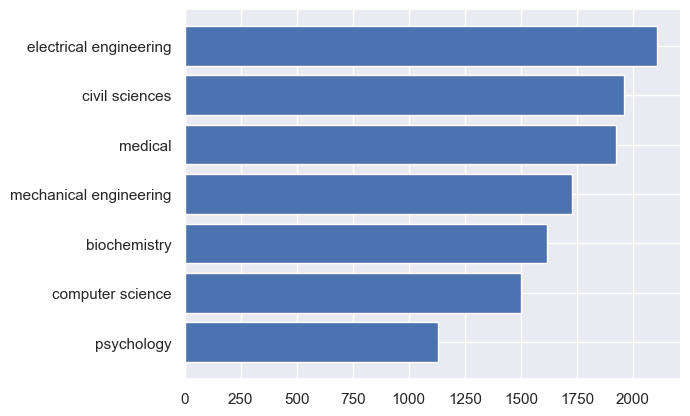
\includegraphics[width=0.8\linewidth]{figs/wos_distrib.png}
    \caption{The class distribution of the sample of the WOS-11967 dataset}
    \label{fig:wos_distrib}
\end{figure}

To conserve resources typically expended on extracting rationales from LLM, I strategically extracted a subset of 4,787 samples from the dataset maintaining the same class distribution as the original. This method not only streamlines the computational demands but also allows for a more focused examination of the model's capability to handle and classify data effectively under conditions of a substantially reduced dataset size.

For the generation of rationales within the dataset, I employed a methodology similar to the one used for the e-SNLI dataset, focusing initially on the creation of two example rationales for each category for few-shot learning with the LLM\@. These rationales were generated by prompting GPT-3.5 using prompt depicted at \autoref{fig:wos_eg_prompt}.

\begin{figure}[ht!]
    \centering
    \lstinputlisting[columns=fullflexible,basicstyle=\small,breaklines=true,breakatwhitespace,breakindent=0em,xleftmargin=1.5cm,xrightmargin=1.5cm,backgroundcolor=\color{lightgray},frame=tlbr,framesep=0.5cm,framerule=0pt]{figs/wos_example_prompt.txt}
    \caption{Prompt for generating example rationales (for few-shot prompting) for the WOS-11967 dataset.}
    \label{fig:wos_eg_prompt}
\end{figure}

After collecting this samples for few-shot learning, I conducted a thorough manual review of each entry. This step was crucial to ensure the quality and consistency of the example shots for the LLM\@.

Using these curated example rationales, I engaged GPT-3.5 in a few-shot learning scenario, where the model was fed with the eamples along prompt to generate rationales.

\begin{figure}[ht!]
    \centering
    \lstinputlisting[columns=fullflexible,basicstyle=\small,breaklines=true,breakatwhitespace,breakindent=0em,xleftmargin=1.5cm,xrightmargin=1.5cm,backgroundcolor=\color{lightgray},frame=tlbr,framesep=0.5cm,framerule=0pt]{figs/wos_prompt.txt}
    \caption{Prompt for generating rationales for the WOS-11967 dataset.}
    \label{fig:wos_prompt}
\end{figure}

This rigorous process ensures that the rationales are not only generated efficiently but are also of high quality and consistent, thereby enhancing the reliability of the dataset for subsequent machine learning tasks.

Resulting dataset consists of 4,787 samples, each annotated with an original label and an LLM-provided rationale. The dataset is available at \linebreak \url{https://huggingface.co/datasets/batalovme/wos_with_rationale}.
